\documentclass[]{article}
\usepackage{lmodern}
\usepackage{amssymb,amsmath}
\usepackage{ifxetex,ifluatex}
\usepackage{fixltx2e} % provides \textsubscript
\ifnum 0\ifxetex 1\fi\ifluatex 1\fi=0 % if pdftex
  \usepackage[T1]{fontenc}
  \usepackage[utf8]{inputenc}
\else % if luatex or xelatex
  \ifxetex
    \usepackage{mathspec}
  \else
    \usepackage{fontspec}
  \fi
  \defaultfontfeatures{Ligatures=TeX,Scale=MatchLowercase}
\fi
% use upquote if available, for straight quotes in verbatim environments
\IfFileExists{upquote.sty}{\usepackage{upquote}}{}
% use microtype if available
\IfFileExists{microtype.sty}{%
\usepackage[]{microtype}
\UseMicrotypeSet[protrusion]{basicmath} % disable protrusion for tt fonts
}{}
\PassOptionsToPackage{hyphens}{url} % url is loaded by hyperref
\usepackage[unicode=true]{hyperref}
\hypersetup{
            pdfborder={0 0 0},
            breaklinks=true}
\urlstyle{same}  % don't use monospace font for urls
\usepackage[margin=1in]{geometry}
\usepackage{color}
\usepackage{fancyvrb}
\newcommand{\VerbBar}{|}
\newcommand{\VERB}{\Verb[commandchars=\\\{\}]}
\DefineVerbatimEnvironment{Highlighting}{Verbatim}{commandchars=\\\{\}}
% Add ',fontsize=\small' for more characters per line
\newenvironment{Shaded}{}{}
\newcommand{\KeywordTok}[1]{\textcolor[rgb]{0.00,0.44,0.13}{\textbf{#1}}}
\newcommand{\DataTypeTok}[1]{\textcolor[rgb]{0.56,0.13,0.00}{#1}}
\newcommand{\DecValTok}[1]{\textcolor[rgb]{0.25,0.63,0.44}{#1}}
\newcommand{\BaseNTok}[1]{\textcolor[rgb]{0.25,0.63,0.44}{#1}}
\newcommand{\FloatTok}[1]{\textcolor[rgb]{0.25,0.63,0.44}{#1}}
\newcommand{\ConstantTok}[1]{\textcolor[rgb]{0.53,0.00,0.00}{#1}}
\newcommand{\CharTok}[1]{\textcolor[rgb]{0.25,0.44,0.63}{#1}}
\newcommand{\SpecialCharTok}[1]{\textcolor[rgb]{0.25,0.44,0.63}{#1}}
\newcommand{\StringTok}[1]{\textcolor[rgb]{0.25,0.44,0.63}{#1}}
\newcommand{\VerbatimStringTok}[1]{\textcolor[rgb]{0.25,0.44,0.63}{#1}}
\newcommand{\SpecialStringTok}[1]{\textcolor[rgb]{0.73,0.40,0.53}{#1}}
\newcommand{\ImportTok}[1]{#1}
\newcommand{\CommentTok}[1]{\textcolor[rgb]{0.38,0.63,0.69}{\textit{#1}}}
\newcommand{\DocumentationTok}[1]{\textcolor[rgb]{0.73,0.13,0.13}{\textit{#1}}}
\newcommand{\AnnotationTok}[1]{\textcolor[rgb]{0.38,0.63,0.69}{\textbf{\textit{#1}}}}
\newcommand{\CommentVarTok}[1]{\textcolor[rgb]{0.38,0.63,0.69}{\textbf{\textit{#1}}}}
\newcommand{\OtherTok}[1]{\textcolor[rgb]{0.00,0.44,0.13}{#1}}
\newcommand{\FunctionTok}[1]{\textcolor[rgb]{0.02,0.16,0.49}{#1}}
\newcommand{\VariableTok}[1]{\textcolor[rgb]{0.10,0.09,0.49}{#1}}
\newcommand{\ControlFlowTok}[1]{\textcolor[rgb]{0.00,0.44,0.13}{\textbf{#1}}}
\newcommand{\OperatorTok}[1]{\textcolor[rgb]{0.40,0.40,0.40}{#1}}
\newcommand{\BuiltInTok}[1]{#1}
\newcommand{\ExtensionTok}[1]{#1}
\newcommand{\PreprocessorTok}[1]{\textcolor[rgb]{0.74,0.48,0.00}{#1}}
\newcommand{\AttributeTok}[1]{\textcolor[rgb]{0.49,0.56,0.16}{#1}}
\newcommand{\RegionMarkerTok}[1]{#1}
\newcommand{\InformationTok}[1]{\textcolor[rgb]{0.38,0.63,0.69}{\textbf{\textit{#1}}}}
\newcommand{\WarningTok}[1]{\textcolor[rgb]{0.38,0.63,0.69}{\textbf{\textit{#1}}}}
\newcommand{\AlertTok}[1]{\textcolor[rgb]{1.00,0.00,0.00}{\textbf{#1}}}
\newcommand{\ErrorTok}[1]{\textcolor[rgb]{1.00,0.00,0.00}{\textbf{#1}}}
\newcommand{\NormalTok}[1]{#1}
\usepackage{graphicx,grffile}
\makeatletter
\def\maxwidth{\ifdim\Gin@nat@width>\linewidth\linewidth\else\Gin@nat@width\fi}
\def\maxheight{\ifdim\Gin@nat@height>\textheight\textheight\else\Gin@nat@height\fi}
\makeatother
% Scale images if necessary, so that they will not overflow the page
% margins by default, and it is still possible to overwrite the defaults
% using explicit options in \includegraphics[width, height, ...]{}
\setkeys{Gin}{width=\maxwidth,height=\maxheight,keepaspectratio}
\IfFileExists{parskip.sty}{%
\usepackage{parskip}
}{% else
\setlength{\parindent}{0pt}
\setlength{\parskip}{6pt plus 2pt minus 1pt}
}
\setlength{\emergencystretch}{3em}  % prevent overfull lines
\providecommand{\tightlist}{%
  \setlength{\itemsep}{0pt}\setlength{\parskip}{0pt}}
\setcounter{secnumdepth}{0}
% Redefines (sub)paragraphs to behave more like sections
\ifx\paragraph\undefined\else
\let\oldparagraph\paragraph
\renewcommand{\paragraph}[1]{\oldparagraph{#1}\mbox{}}
\fi
\ifx\subparagraph\undefined\else
\let\oldsubparagraph\subparagraph
\renewcommand{\subparagraph}[1]{\oldsubparagraph{#1}\mbox{}}
\fi

% set default figure placement to htbp
\makeatletter
\def\fps@figure{htbp}
\makeatother


\date{}

\begin{document}

\section{Vulnerability Documentation}\label{vulnerability-documentation}

This is the documentation to test vulnerabilities in password managers
found in the paper
\href{https://www.overleaf.com/read/rkvzgttqvmkk}{Analysis on the
Security and Use of Password Managers}. We have found five successful
attacks that exploit vulnerabilities in Passbolt, Padlock and Encryptr.

\subsubsection{Attacks}\label{attacks}

\begin{itemize}
\tightlist
\item
  \protect\hyperlink{userscripts}{Userscripts}
\item
  \protect\hyperlink{installing-scripts}{Installing Scripts}
\item
  \protect\hyperlink{passbolt-fake-extension-installer}{Passbolt Fake
  Extension Installer}
\item
  \protect\hyperlink{padlock-data-reset}{Padlock Data Reset}

  \begin{itemize}
  \tightlist
  \item
    \protect\hyperlink{padlock-application-setup}{Padlock Application
    Setup}
  \item
    \protect\hyperlink{resetting}{Resetting}
  \item
    \protect\hyperlink{resync}{Resync}
  \item
    \protect\hyperlink{testing-script}{Testing Script}
  \end{itemize}
\item
  \protect\hyperlink{padlock-access-remover}{Padlock Access Remover}

  \begin{itemize}
  \tightlist
  \item
    \protect\hyperlink{padlock-application-setup-1}{Padlock Application
    Setup}
  \item
    \protect\hyperlink{testing-script-1}{Testing Script}
  \end{itemize}
\item
  \protect\hyperlink{user-input-attacks}{User Input Attacks}
\item
  \protect\hyperlink{keylogger-attack}{Keylogger Attack}
\item
  \protect\hyperlink{clipboard-reader}{Clipboard Reader}
\item
  \protect\hyperlink{usage}{Usage}

  \begin{itemize}
  \tightlist
  \item
    \protect\hyperlink{installation}{Installation}
  \item
    \protect\hyperlink{setup}{Setup}
  \item
    \protect\hyperlink{stopping-the-program}{Stopping the Program}
  \end{itemize}
\end{itemize}

\hypertarget{userscripts}{\subsection{Userscripts}\label{userscripts}}

Before you start using any of the userscript attacks, you need to use a
userscript manager.

For Chrome, use \href{https://tampermonkey.net/}{Tampermonkey}.

For Firefox, use
\href{https://addons.mozilla.org/en-US/firefox/addon/greasemonkey/}{Greasemonkey}.

\hypertarget{installing-scripts}{\subsubsection{Installing
Scripts}\label{installing-scripts}}

Tampermonkey and Greasemonkey should automatically install the
userscripts when you click the given install link. If you have trouble
installing any userscript look at the wiki for your userscript manager.

Tampermonkey - \url{https://tampermonkey.net/faq.php\#Q102}

Greasemonkey -
\url{https://wiki.greasespot.net/Greasemonkey_Manual:Installing_Scripts}

Firefox is preferred because all the scripts will execute fully on
Firefox.

\hypertarget{passbolt-fake-extension-installer}{\subsubsection{Passbolt
Fake Extension Installer}\label{passbolt-fake-extension-installer}}

\href{https://github.com/iblacksand/VulnerabilityDocumentation/raw/master/PassboltFakeExtensionInstall.user.js}{\textbf{Install}}

\textbf{MAKE SURE YOU REMOVE ALL OTHER USERSCRIPTS OR ELSE IT MAY NOT
WORK}

This script will change all links that download the passbolt extension
to download a random script (we chose
\href{https://addons.mozilla.org/en-US/firefox/addon/noscript/}{NoScript}).
For this to work you need to use Firefox (See
\protect\hyperlink{userscripts}{Userscripts} for more info).

After you install the program, you can use your own Passbolt server
(look at Passbolt's
\href{https://medium.com/passbolt/passbolt-on-debian-8-71-from-scratch-4438dad18908}{medium
blog} for a tutorial on how to set it up), or you can use
\href{https://demo.passbolt.com}{Passbolt's demo server}. Make sure that
you \textbf{don't} have Passbolt's extension installed, or else no links
will show.

\begin{enumerate}
\def\labelenumi{\arabic{enumi}.}
\item
  Go to your server's login page (For Passbolt's demo this is
  \href{https://demo.passbolt.com}{demo.passbolt.com}).
\item
  Hover over the link that says \texttt{Download\ it\ here}.
\end{enumerate}

\begin{figure}
\centering
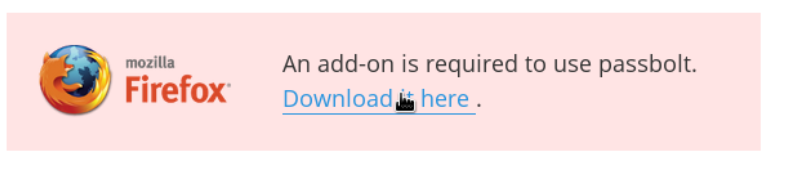
\includegraphics{images/PassboltExt-04.png}
\caption{Hover over link}
\end{figure}

\begin{enumerate}
\def\labelenumi{\arabic{enumi}.}
\setcounter{enumi}{2}
\tightlist
\item
  Look at the bottom left and notice that Firefox says the link goes to
  \texttt{https://www.passbolt.com/download/firefox}
\end{enumerate}

\begin{figure}
\centering
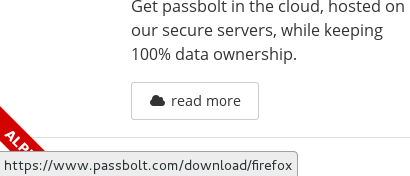
\includegraphics{images/PassboltExt-01.png}
\caption{Firefox shows link still is Passbolt}
\end{figure}

\begin{enumerate}
\def\labelenumi{\arabic{enumi}.}
\setcounter{enumi}{3}
\tightlist
\item
  Click on the link and press allow on the Firefox popup.
\end{enumerate}

\begin{figure}
\centering
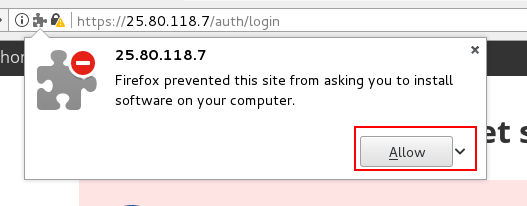
\includegraphics{images/PassboltExt-05.png}
\caption{Allow server to install extension}
\end{figure}

\begin{enumerate}
\def\labelenumi{\arabic{enumi}.}
\setcounter{enumi}{4}
\tightlist
\item
  Notice how Firefox is installing \texttt{Noscript} Rather than
  \texttt{Passbolt}.
\end{enumerate}

\begin{figure}
\centering
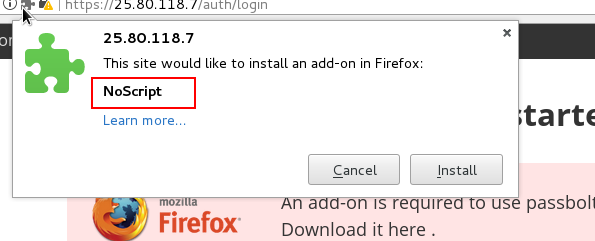
\includegraphics{images/PassboltExt-06.png}
\caption{Downloads NoScript instead of Passbolt}
\end{figure}

The script made the link look like it was downloading a link from
Passbolt but it changed the link to download a different link. This
extension could have the logo and name of Passbolt and the user will be
unlikely to see any foul play.

If the script didn't work or there was problem testing,
\href{https://github.com/iblacksand/VulnerabilityDocumentation/issues}{open
an issue} and we will come back to you.

\hypertarget{padlock-data-reset}{\subsubsection{Padlock Data
Reset}\label{padlock-data-reset}}

\href{https://github.com/iblacksand/VulnerabilityDocumentation/raw/master/PadlockButtonClick.user.js}{\textbf{Install}}

\textbf{MAKE SURE YOU REMOVE ALL OTHER USERSCRIPTS OR ELSE IT MAY NOT
WORK}

This script will automatically reset all data on a Padlock account.

\hypertarget{padlock-application-setup}{\paragraph{Padlock Application
Setup}\label{padlock-application-setup}}

You first need to install Padlock and get the cloud connected. You can
download Padlock \href{http://padlock.io/}{here}. You can use the
Padlock cloud \href{https://cloud.padlock.io/login/}{here}, which is on
a 30 day trial, or you can use your own Padlock cloud which you can
install from \href{https://github.com/maklesoft/padlock-cloud}{here}. If
you use a custom server, you can check out my
\href{https://github.com/iblacksand/custompadlock}{custompadlock repo}
which is a custom application that will allow the application to use
\texttt{http://} so you don't have to get a certificate.

\emph{If you used my custom padlock application then the layout is not
exactly the same but the steps are basically the same. I use the most
updated version of padlock but the application on the official website
is behind}

Once you get your cloud and program running, go to the Padlock
application itself. Log in to your account, and get to page that has
\texttt{Import\ Data,\ Synchronize\ and\ Create\ Record}. Click on
\texttt{Synchronize\ data\ \textgreater{}\ Open\ Padlock\ Cloud\ Settings}.
If you use a custom server click on
\texttt{use\ custom\ server\ \textgreater{}\ continue} and enter the IP
of your server. Next press \texttt{get\ started} and then enter in your
email (You can use a service like
\href{https://www.guerrillamail.com/}{Guerrilla Mail} to make multiple
accounts). Then press \texttt{connect}. Go into your email and you
should receive an email with a link. Click on the link and your
application should be synced with the cloud. You can check this by
clicking \texttt{synchronize} on the application. The application should
say that it synced correctly. You can go back to the application and
press the \texttt{\textless{}} in the top left twice until you get back
to the screen with
\texttt{Import\ Data,\ Synchronize\ and\ Create\ Record}. Click
\texttt{Create\ Record} and enter an example name, like
\texttt{test\ name} and then press \texttt{add}. Click on the box with
\texttt{username} then click \texttt{edit}. You can now enter in an
example username like \texttt{testusername}. Then click anywhere outside
of the text box. Now click the box with \texttt{password} then click
\texttt{Edit}. Enter in a password like \texttt{testpassword}. Then
click anywhere outside of the box. Your screen should know look like

\begin{figure}
\centering
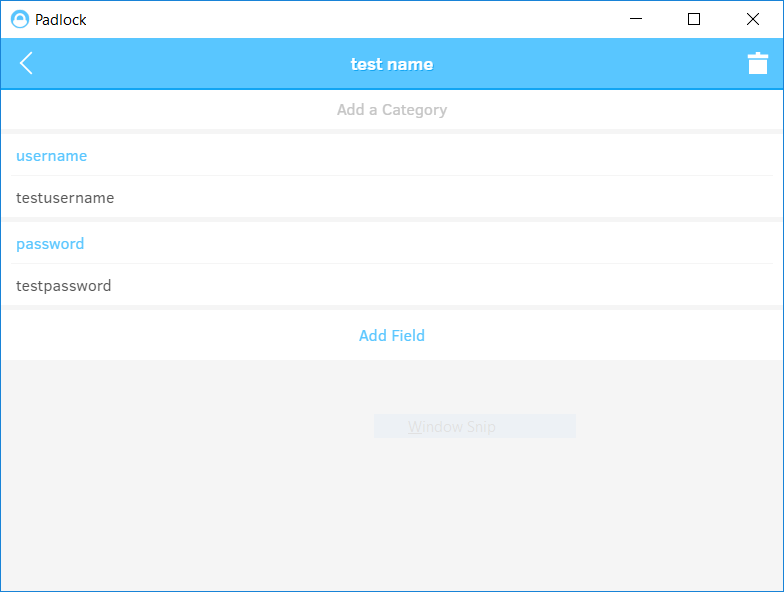
\includegraphics{images/Padlock-01.png}
\caption{}
\end{figure}

You can press on the top left \texttt{\textless{}} and then click on the
three lines in the top left. Then click on \texttt{synchronize}. The
bottom of the application should say application should say that it
synchronized correctly. Next you need to test the syncing to ensure that
the steps for testing the userscript should work. First, you need to
reset the app

\hypertarget{resetting}{\subparagraph{Resetting}\label{resetting}}

To reset the application go to the screen that looks like

\begin{figure}
\centering
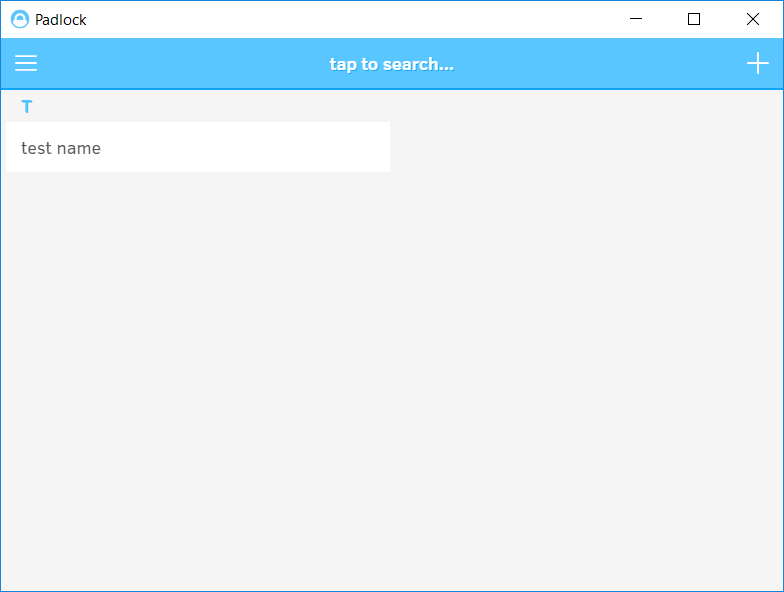
\includegraphics{images/Padlock-02.png}
\caption{padlock}
\end{figure}

Click on the the three lines in the top left and then click
\texttt{settings}. Next click \texttt{reset\ app}. Enter your master
password and then your application should be reset.

\hypertarget{resync}{\subparagraph{Resync}\label{resync}}

After, resetting, create a new master password and log back into
Padlock. You should see a menu with
\texttt{Import\ Data,\ Synchronize\ and\ Create\ Record}. Click on
\texttt{synchronize} and use the same email and server that you used
before. Click on \texttt{get\ started}, enter your email, and go to your
inbox. When you receive an email with the link, click on it and the
application should be synced. After you click the link, go to the
Padlock application and click on \texttt{synchronize} or
\texttt{synchronize\ now} (whichever pops up). If you go to where your
records are stored (press the \texttt{\textless{}} in the top left until
you see it), you should see the entry we made earlier.

\begin{figure}
\centering
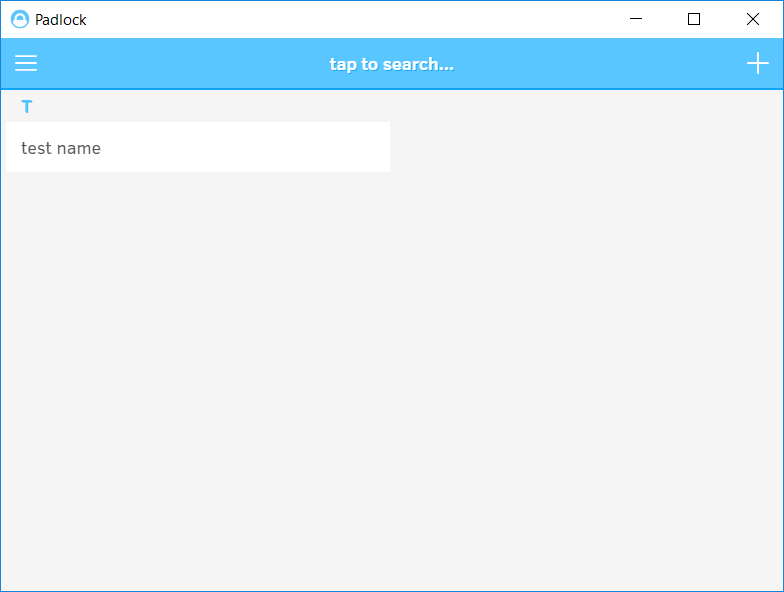
\includegraphics{images/Padlock-02.png}
\caption{Padlock}
\end{figure}

If you see something similar to this, then you have succesfully synced
Padlock to the cloud!

If you had a problem with the above,
\href{https://github.com/iblacksand/VulnerabilityDocumentation/issues}{open
an issue} and we will come back to you.

\hypertarget{testing-script}{\paragraph{Testing
Script}\label{testing-script}}

To test the script, install the script with the link given above (See
\protect\hyperlink{installing-scripts}{installing scripts}).

Once you install the script make sure you have usernames and passwords
stored in the cloud (this is done in
\protect\hyperlink{padlock-application-setup}{padlock application
setup}). Now reset your application (see
\protect\hyperlink{resetting}{resetting}).

Next, log in to the dashboard for the cloud server that you used with
the script active. To do this, go to the url of your server. For the
padlock cloud this is at
\href{https://cloud.padlock.io/}{cloud.padlock.io}. Use the email you
used in the setup and a link should be given to your email.

Upon clicking the link, the userscript will autoclick things on the
screen so the page will change. Make sure that the script is active
before you click the link.

Depending on your computer, the website will change 1-10 times. This is
dependent on when the script and buttons load on the screen. When the
website stops changing the top of your screen should show
\texttt{Your\ data\ has\ been\ reset\ successfully!}.

\begin{figure}
\centering
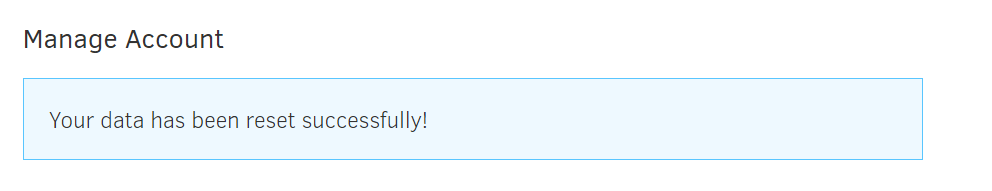
\includegraphics{images/Padlock-03.png}
\caption{Padlock}
\end{figure}

Now resync your padlock application (see
\protect\hyperlink{resync}{resync} for the steps). Upon resync, you
should see that no entries are restored. All the data has been cleared.

If the script didn't work or there was problem testing,
\href{https://github.com/iblacksand/VulnerabilityDocumentation/issues}{open
an issue} and we will come back to you.

\hypertarget{padlock-access-remover}{\subsubsection{Padlock Access
Remover}\label{padlock-access-remover}}

\href{https://github.com/iblacksand/VulnerabilityDocumentation/raw/master/PadlockAutoFormSubmit.user.js}{\textbf{INSTALL}}

\textbf{MAKE SURE YOU REMOVE ALL OTHER USERSCRIPTS OR ELSE IT MAY NOT
WORK}

\hypertarget{padlock-application-setup-1}{\paragraph{Padlock Application
Setup}\label{padlock-application-setup-1}}

See \protect\hyperlink{padlock-application-setup}{Padlock Application
Setup} above.

\hypertarget{testing-script-1}{\paragraph{Testing
Script}\label{testing-script-1}}

To test the script, install the script with the link given above (See
\protect\hyperlink{installing-scripts}{installing scripts}).

Make sure that you went through all the steps of
\protect\hyperlink{padlock-application-setup}{Padlock Application
Setup}.

Next, log in to the dashboard for the cloud server that you used with
the script active. To do this, go to the url of your server. For the
padlock cloud this is at
\href{https://cloud.padlock.io/}{cloud.padlock.io}. Use the email you
used in the setup and a link should be given to your email.

Upon clicking the link, the userscript will autoclick things on the
screen so the page will change. Make sure that the script is active
before you click the link.

Once you click the link, you might end up at
\texttt{https://cloud.padlock.io/subscribe/} with a page saying
\texttt{Bad\ Request:\ No\ stripe\ token\ provided}. This is normal. Go
back to the application. You should see a message saying
\texttt{It\ seems\ you\ have\ disconnected\ from\ Padlock\ C.loud.\ Please\ reconnect\ ...}.
The script revoked your access to your account, but it did not reset
your data.

If the script didn't work or there was problem testing,
\href{https://github.com/iblacksand/VulnerabilityDocumentation/issues}{open
an issue} and we will come back to you.

\hypertarget{user-input-attacks}{\subsection{User Input
Attacks}\label{user-input-attacks}}

Both user input attacks were built in C\# for use only on Windows
devices. They work in much the same way. Both of the attacks save
plain-text logs with timestamps. Every 10 minutes, the attacks send the
logs to our email and delete them from the victim's computer.

\hypertarget{keylogger-attack}{\subsubsection{Keylogger
Attack}\label{keylogger-attack}}

The keylogger saves every key press and click into a plain-text file. It
attaches a timestamp at the beginning of each log and after 30 seconds
of inactivity.

\hypertarget{clipboard-reader}{\subsubsection{Clipboard
Reader}\label{clipboard-reader}}

The clipboard reader checks four times every second to see if the
contents of the clipboard have changed. Every time it detects a change,
it logs the timestamp and clipboard contents.

\hypertarget{usage}{\subsubsection{Usage}\label{usage}}

\hypertarget{installation}{\paragraph{Installation}\label{installation}}

Both of these attacks can be hidden in the installation of a different
(seemingly safe) program and set up to run every time Windows boots up.
Additionally, anyone with access to a victim's computer could install
it. For our purposes, we combined both attacks into a single
installation. If you'd like to view the source code and/or build it
yourself, click
\href{https://github.com/Guzaboo/KeyloggerExample/tree/master}{here}.

In order to test, first
\href{https://github.com/iblacksand/VulnerabilityDocumentation/releases}{go
to this link} and download one of the below files:

\begin{itemize}
\tightlist
\item
  Manual-start program: download loggers.zip
\item
  Windows-startup installer: download setup.exe
\end{itemize}

If you download the manual-start, unzip the file and skip to
\protect\hyperlink{setup}{Setup}

If you download the installer, the files will be saved in the following
location:\\
\texttt{C:\textbackslash{}Users\textbackslash{}\textless{}WINDOWS\ ACCOUNT\ NAME\textgreater{}\textbackslash{}AppData\textbackslash{}Local\textbackslash{}Fake\ Microsoft\ Process}

\hypertarget{setup}{\paragraph{Setup}\label{setup}}

In the folder where you saved the file should be a file called
config.json\\
Enter in your email and password. The program will send you emails from
yourself with the logs attached. You must use a gmail account. Example:

\begin{Shaded}
\begin{Highlighting}[]
\FunctionTok{\{}
    \DataTypeTok{"email"}\FunctionTok{:} \StringTok{"exampleaccount@gmail.com"}\FunctionTok{,}
    \DataTypeTok{"password"}\FunctionTok{:} \StringTok{"examplePassw0rd"}
\FunctionTok{\}}
\end{Highlighting}
\end{Shaded}

Next you must click this link and
\href{https://myaccount.google.com/lesssecureapps?rfn=27\&rfnc=1\&eid=1003975247538190077\&et=0\&asae=2\&pli=1}{allow
less secure apps}.

Now double click temps.exe to run the program. For testing purposes we
have set the program to email you every 40 seconds instead of 10
minutes, so type, copy/paste, etc and check your email after 40 seconds.

\hypertarget{stopping-the-program}{\paragraph{Stopping the
Program}\label{stopping-the-program}}

When you are done testing, press \texttt{Ctrl\ +\ Alt\ +\ Delete} to
open Task Manager. Look for \texttt{temps} under background processes
and end the process.

\textbf{If you used the Windows-startup installer} and you want to
remove it from your startup processes, press
\texttt{Ctrl\ +\ Alt\ +\ Delete} to open Task Manager. Click on the
\texttt{Startup} tab on the top bar of Task Manager. Click on
\texttt{temps} and click \texttt{Disable}.

\end{document}
